\begin{figure}[htbp]
\section*{ UMOD}
\centering
\begin{subfigure}[b]{0.45\textwidth}
\centering
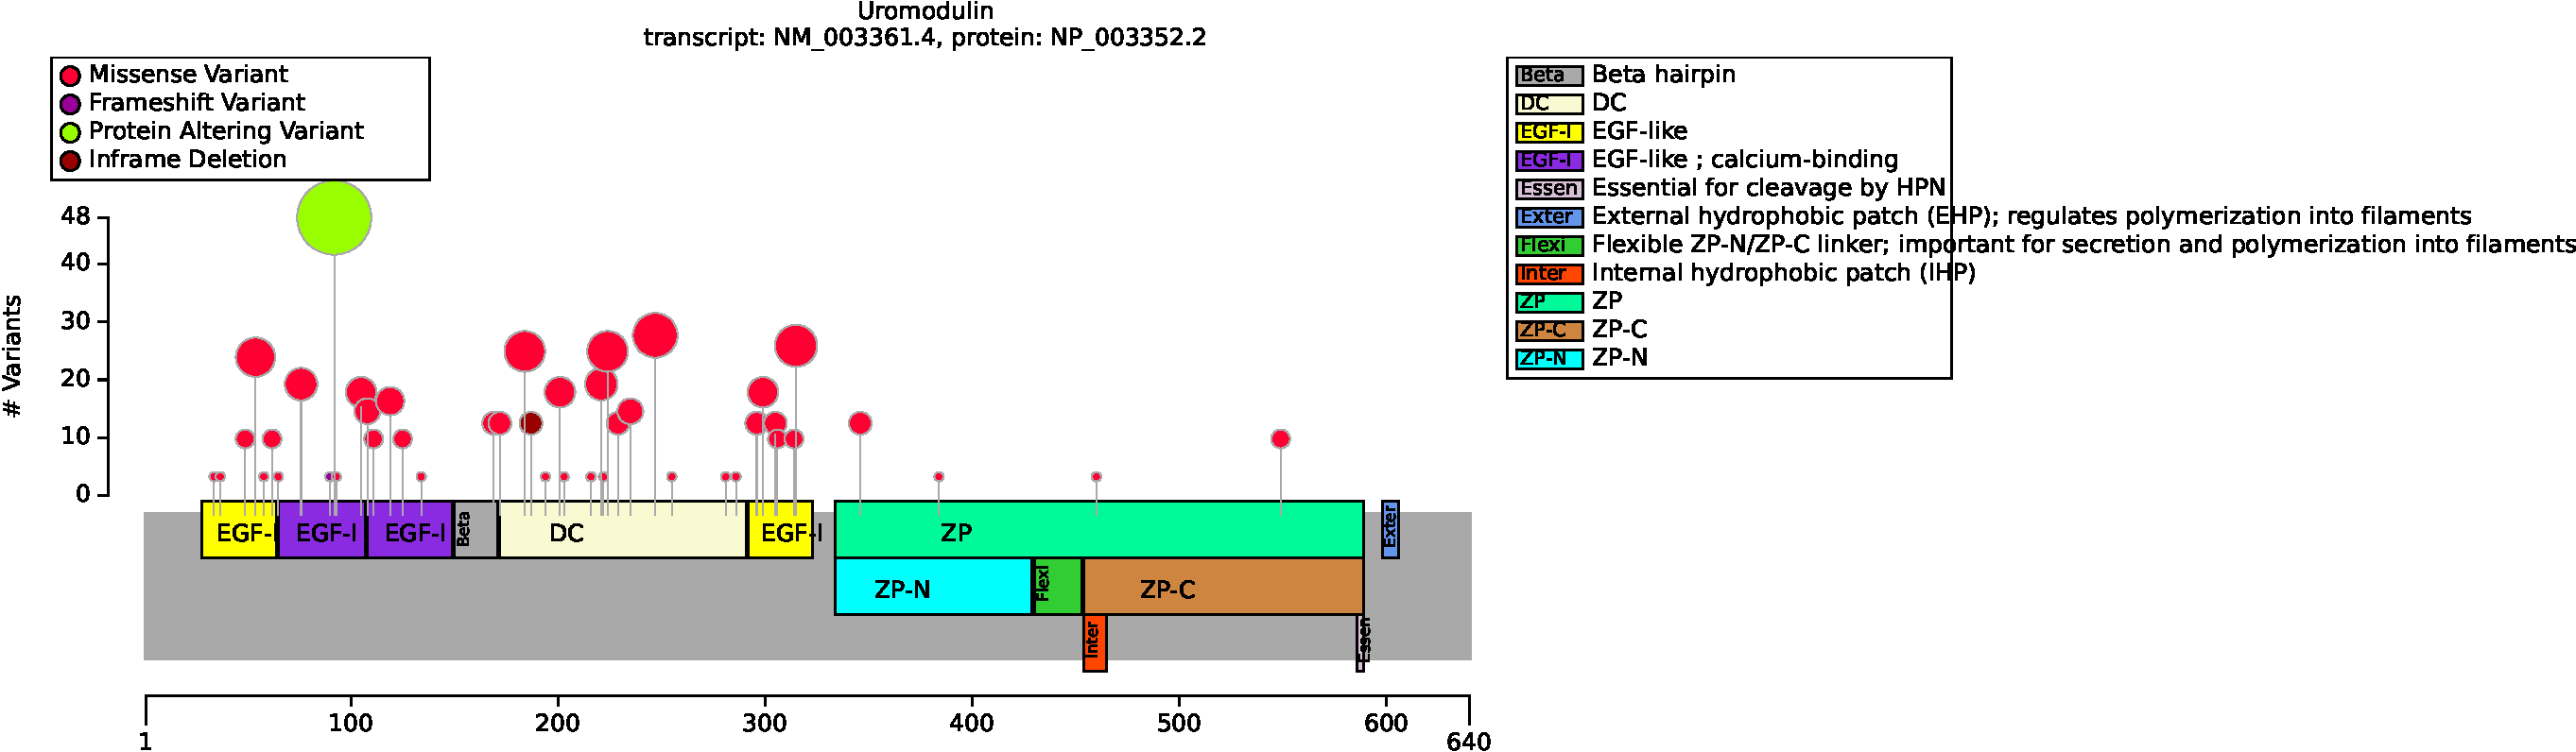
\includegraphics[width=\textwidth]{img/UMOD_protein_diagram.pdf} 
\captionsetup{justification=raggedright,singlelinecheck=false}
\caption{Distribution of variants in UMOD}
\end{subfigure}
\begin{subfigure}[b]{0.45\textwidth}
\centering
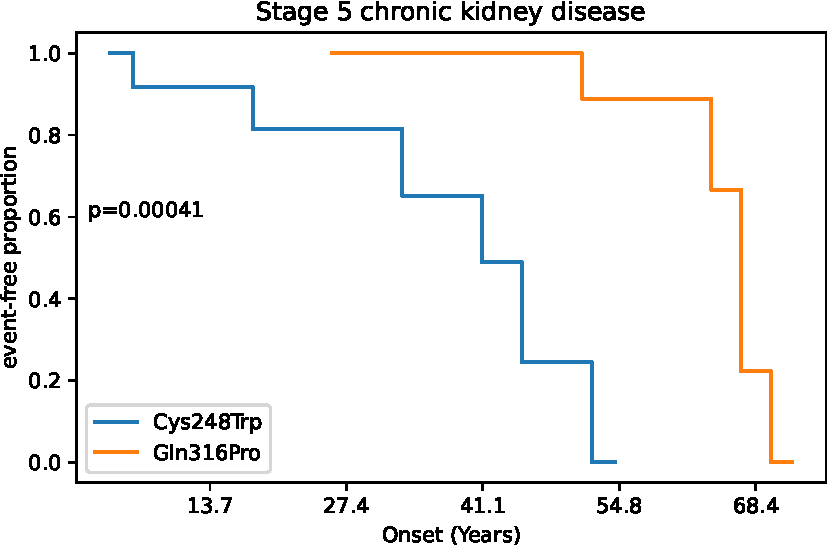
\includegraphics[width=\textwidth]{ img/UMOD_stats.pdf} 
\captionsetup{justification=raggedright,singlelinecheck=false}
\caption{Onset of
Stage 5 chronic kidney disease (HP:0003774)}
\end{subfigure}

\vspace{1em}

\begin{subfigure}[b]{0.95\textwidth}
\centering
\resizebox{\textwidth}{!}{
\begin{tabular}{llllrr}
\toprule
HPO term & EGF & other & p-value & adj. p-value\\
\midrule
Hyperuricemia [HP:0002149] & 14/32 (44\%) & 50/57 (88\%) & $1.77\times 10^{-5}$ & $1.06\times 10^{-4}$\\
\bottomrule
\end{tabular}
}
\captionsetup{justification=raggedright,singlelinecheck=false}
\caption{Fisher Exact Test: HPO annotation frequency and EGF vs. other. Total of 6 tests were performed. }
\end{subfigure}

\begin{subfigure}[b]{0.95\textwidth}
\centering
\resizebox{\textwidth}{!}{
\begin{tabular}{llllrr}
\toprule
HPO term & cysteine & other & p-value & adj. p-value\\
\midrule
Hyperuricemia [HP:0002149] & 38/41 (93\%) & 26/48 (54\%) & $4.48\times 10^{-5}$ & $2.69\times 10^{-4}$\\
\bottomrule
\end{tabular}
}
\captionsetup{justification=raggedright,singlelinecheck=false}
\caption{Fisher Exact Test: HPO annotation frequency and cysteine vs other. Total of  6 tests were performed. }
\end{subfigure}

\begin{subfigure}[b]{0.95\textwidth}
\centering
\resizebox{\textwidth}{!}{
\begin{tabular}{llllrr}
\toprule
Genotype (A) & Genotype (B) & total tests performed & significant results\\
\midrule
FEMALE & MALE & 5 & 0\\
\bottomrule
\end{tabular}
}
\captionsetup{justification=raggedright,singlelinecheck=false}
\caption{Fisher Exact Test performed to compare HPO annotation frequency with respect to genotypes. }
\end{subfigure}
\vspace{2em}

\begin{subfigure}[b]{0.95\textwidth}
\captionsetup{justification=raggedright,singlelinecheck=false}
\resizebox{\textwidth}{!}{
\begin{tabular}{llllrr}
\toprule
Description & Variable & Genotype (A) & Genotype (B) & p-value & xrefs\\
\midrule
Survival analysis: Stage 5 chronic kidney disease & Onset of HP:0003774 & EGF & other & 0.284 & -\\
\bottomrule
\end{tabular}
}
\caption{ Onset of Stage 5 chronic kidney disease to compare EGF and other with respect to Onset of HP:0003774. }
\end{subfigure}

\vspace{2em}

\begin{subfigure}[b]{0.95\textwidth}
\captionsetup{justification=raggedright,singlelinecheck=false}
\resizebox{\textwidth}{!}{
\begin{tabular}{llllrr}
\toprule
Description & Variable & Genotype (A) & Genotype (B) & p-value & xrefs\\
\midrule
Survival analysis: Stage 5 chronic kidney disease & Onset of HP:0003774 & 278_289delins & other & 0.835 & -\\
\bottomrule
\end{tabular}
}
\caption{ Onset of Stage 5 chronic kidney disease to compare 278_289delins and other with respect to Onset of HP:0003774. }
\end{subfigure}

\vspace{2em}
\begin{subfigure}[b]{0.95\textwidth}
\captionsetup{justification=raggedright,singlelinecheck=false}
\resizebox{\textwidth}{!}{
\begin{tabular}{llllrr}
\toprule
Description & Variable & Genotype (A) & Genotype (B) & p-value & xrefs\\
\midrule
Survival analysis: Stage 5 chronic kidney disease & Onset of HP:0003774 & Cys248Trp & Gln316Pro & $4.10\times 10^{-4}$ & -\\
\bottomrule
\end{tabular}
}
\caption{ Onset of Stage 5 chronic kidney disease to compare Cys248Trp and Gln316Pro with respect to Onset of
Stage 5 chronic kidney disease (HP:0003774). }
\end{subfigure}

\caption{ The cohort comprised 207 individuals (80 females, 88 males, 39 with unknown sex). 30 HPO terms were used to annotate the cohort. 
Disease diagnoses: Tubulointerstitial kidney disease, autosomal dominant, 1 (OMIM:162000) (183 individuals), 
Tubulointerstitial kidney disease, autosomal dominant, 3 (OMIM:162002) (12 individuals), 
Tubulointerstitial kidney disease, autosomal dominant, 2 (OMIM:162001) (12 individuals). 
One study on UMOD variants showed that median ages at ESRD development were lowest with Cys77Tyr 
and highest with Gln316Pro \cite{PMID_23723338}, which is compatible with our finding here. Another showed that
indel mutation p.Val93\_Gly97delinsAlaAlaSerCys is associated with a relatively mild clinical UAKD phenotype \cite{PMID_22034507}. We did
not observe a significant association between this variant and age of onset with our dataset. 
A total of 53 unique variant alleles were found in \textit{UMOD} (transcript: \texttt{NM\_003361.4}, protein id: \texttt{NP\_003352.2}).}
\end{figure}
